\documentclass[11pt]{beamer}

\usepackage{slides}

\begin{document}

\begin{frame}
	\maketitle
\end{frame}

\begin{section}{Introduction}

\begin{frame}{Introduction: Types of Contact Tracing}
\begin{itemize}
  \item Digital contact tracing (DCT)
  \item Proximity tracing
  \item Decentralized DCT
    \begin{itemize}
      \item Broadcast model
      \item Message-oriented model
    \end{itemize}
\end{itemize}
\end{frame}

\begin{frame}{Introduction: Limitations of Other Approaches}
\begin{itemize}
  \item No DCT approach exists that incorporates both non-diagnostic information and indirect contacts to estimate infection risk.
  \item Accounting for indirect contact can substantially improve the efficacy of DCT \citep{PozoMartin2023}.
  \item \citet{Cherini2023} propose exchanging pseudonyms of indirect contacts, but restrict themselves to diagnostic testing.
  \item \citet{Gupta2023} incorporate non-diagnostic information, but do not account for indirect contact.
\end{itemize}
\end{frame}

\begin{frame}{Introduction: ShareTrace}
\begin{itemize}
  \item Accounts for both non-diagnostic information and indirect contact to estimate infection risk.
  \item Developed in collaboration with Dataswyft \citep{Ayday2020}. 
  \item \citet{Ayday2021} designed ShareTrace to use proximity tracing for contact discovery.
    \begin{itemize}
      \item In practice, this was infeasible, because Apple and Google's Exposure Notification API did not permit the user's ephemeral identifiers to be stored remotely in a Dataswyft Personal Data Store.
    \end{itemize}
\end{itemize}
\end{frame}

\begin{frame}{Introduction: Prior Designs and Implementations}
\begin{itemize}
  \item  ``Thinking like a vertex'' with Apache Giraph
  \item Factor subgraph actors
  \item Driver-monitor-worker framework
  \item Projected subgraph actors \citep{Tatton2022b}
  \item Contact search
\end{itemize}
\end{frame}

\end{section}

\begin{section}{Proposed Design}

\begin{frame}{Proposed Design: Definitions}
\begin{itemize}
  \item \define{Risk score}, $\vScore_\vTime \in [0, 1]$: a timestamped infection probability where $\vTime \in \naturals$ is the time of its computation
  \item \define{Symptom score}: prior infection probability; accounts for an individual's demographics, symptoms, and diagnosis \citep{Briers2020, Menni2020}
  \item \define{Exposure score}: posterior infection probability; accounts for direct and indirect contact with others
\end{itemize}
\end{frame}

\begin{frame}{Synchronous Risk Propagation}
\begin{function}{\nRiskPropagation}[\vScores, \vContacts]
  \State{$\vRiskScores{i}{n - 1} \assign \topK{\vScores_i}$}
  \pause
  \State $\vExposureScore{i}{n - 1} \assign \max \vRiskScores{i}{n - 1}$
  \pause
  \State $\vExposureScore{i}{n} \assign \infty$
  \pause
  \While{$\| \vExposureScores{n} - \vExposureScores{n - 1} \| > \pDiff$}
  \pause
    \State $\vVariableMessage{i}{j}{n} \assign \vRiskScores{i}{n - 1} \setminus \setBuilder{\vFactorMessage{j}{i}{\ell}}{\ell \in \intInterval{1}{n - 1}}$
    \pause
    \State $\vFactorMessage{i}{j}{n} \assign \max \setBuilder{\pTransmissionRate \vScore_\vTime}{\vScore_\vTime \in \vVariableMessage{i}{j}{n}, \vTime < \vTime_{ij} + \pTimeBuffer}$
    \pause
    \State $\vRiskScores{i}{n} \assign \topK{\setBuilder{\vFactorMessage{j}{i}{n}}{\vFactor[ij] \in \vNeighbors_i}}$
    \pause
    \State $\vExposureScore{i}{n} \assign \max \vRiskScores{i}{n}$
    \pause
  \EndWhile
  \State \Return $\vExposureScores{n}$
\end{function}
\end{frame}

\begin{frame}{Asynchronous Risk Propagation}
\begin{function}{\nCreateActor}
  \State $\aActorContacts \assign \emptyset$
  \State $\aActorScores \assign \emptyset$
  \State $\aActorExposure \assign \cNullRiskScore$
  \State \Return $\vActor$
\end{function}
\begin{function}{\nNullRiskScore}
  \State $\aScoreValue \assign 0$
  \State $\aScoreTime \assign 0$
  \State \Return $\vScore$
\end{function}
\end{frame}

\begin{frame}{Asynchronous Risk Propagation}
\begin{function}{\nRiskScoreTtl}[\vScore]
  \State \Return $\pScoreExpiry - (\vReferenceTime - \aScoreTime)$
\end{function}
\begin{function}{\nContactTtl}[\vContact]
  \State \Return $\pContactExpiry - (\vReferenceTime - \aContactTime)$
\end{function}
\end{frame}

\begin{frame}{Asynchronous Risk Propagation}
\begin{function}{\nHandleRiskScore}[\vActor, \vScore]
  \If{$\cRiskScoreTtl[\vScore] > 0$}
    \pause
    \State $\aScoreKey \assign [\aScoreTime, \aScoreTime + \pScoreExpiry)$
    \pause
    \State $\cMerge[\aActorScores, \vScore]$
    \pause
    \State $\cUpdateExposureScore[\vActor, \vScore]$
    \pause
    \ForEach{$\vContact \in \aActorContacts$}
      \State $\cApplyRiskScore[\vActor, \vContact, \vScore]$
    \EndFor
  \EndIf
\end{function}
\end{frame}

\begin{frame}{Asynchronous Risk Propagation}
\begin{function}{\nUpdateExposureScore}[\vActor, \vScore]
  \If{$\aActorExposureValue < \aScoreValue$}
    \pause
    \State $\aActorExposure \assign \vScore$
  \pause
  \ElsIf{$\cRiskScoreTtl[\aActorExposure] \leq 0$}
    \pause
    \State $\aActorExposure \assign \cMaximum[\aActorScores]$
  \EndIf
\end{function}
\end{frame}

\begin{frame}{Asynchronous Risk Propagation}
\begin{function}{\nApplyRiskScore}[\vActor, \vContact, \vScore]
  \If{$\aContactTime + \pTimeBuffer > \aScoreTime$}
    \pause
    \State $\aNewScoreValue \assign \pTransmissionRate \cdot \aScoreValue$
    \pause
    \State $\cSend[\aContactName, \vNewScore]$
  \EndIf
\end{function}
\end{frame}

\begin{frame}{Asynchronous Risk Propagation}
\begin{function}{\nSetSendThreshold}[\vContact, \vScore]
  \State $\aNewScoreValue \assign \pSendCoefficient \cdot \aScoreValue$
  \pause
  \State $\aContactThreshold \assign \vNewScore$
\end{function}
\end{frame}

\begin{frame}{Asynchronous Risk Propagation}
\begin{function}{\nUpdateSendThreshold}[\vActor, \vContact]
  \If{$\aContactThresholdValue > 0$}
    \pause
    \If{$\cRiskScoreTtl[\aContactThreshold] \leq 0$}
      \pause
      \State $\vScore \assign \cMaximumOlderThan[\aActorScores, \aContactTime + \pTimeBuffer]$
        \pause
      \State $\aNewScoreValue \assign \pTransmissionRate \cdot \aScoreValue$
        \pause
      \State $\cSetSendThreshold[\vContact, \vNewScore]$
    \EndIf
  \EndIf
\end{function}
\end{frame}

\begin{frame}{Asynchronous Risk Propagation}
\begin{function}{\nApplyRiskScore}[\vActor, \vContact, \vScore]
  \State $\cUpdateSendThreshold[\vActor, \vContact]$
  \pause
  \If{$\aContactThresholdValue < \aScoreValue \AND \aContactTime + \pTimeBuffer > \aScoreTime$}
    \pause
    \State $\aNewScoreValue \assign \pTransmissionRate \cdot \aScoreValue$
    \pause
    \State $\cSetSendThreshold[\vContact, \vNewScore]$
    \pause
    \State $\aContactBuffered \assign \vNewScore$
  \EndIf
\end{function}
\end{frame}

\begin{frame}{Asynchronous Risk Propagation}
\begin{function}{\nHandleFlushTimeout}[\vActor]
  \ForEach{$\vContact \in \aActorContacts$}
    \pause
    \If{$\aContactBuffered \notEquals \nil$}
      \pause
      \State $\cSend[\aContactName, \aContactBuffered]$
      \pause
      \State $\aContactBuffered \assign \nil$
    \EndIf
    \pause
    \If{$\cContactTtl[\vContact] \leq 0$}
      \State $\cDelete[\aActorContacts, \vContact]$
    \EndIf
  \EndFor
\end{function}
\end{frame}

\begin{frame}{Asynchronous Risk Propagation}
\begin{function}{\nHandleContact}[\vActor, \vContact]
  \If{$\cContactTtl[\vContact] > 0$}
    \pause
    \State $\aContactThreshold \assign \cNullRiskScore$
    \pause
    \State $\aContactBuffered \assign \nil$
    \pause
    \State $\aContactKey \assign \aContactName$
    \pause
    \State $\cMerge[\aActorContacts, \vContact]$
    \pause
    \State $\vScore \assign \cMaximumOlderThan[\aActorScores, \aContactTime + \pTimeBuffer]$
    \pause
    \State $\cApplyRiskScore[\vActor, \vContact, \vScore]$
  \EndIf
\end{function}
\end{frame}

\end{section}

\begin{section}{Evaluation}

\begin{frame}[allowframebreaks]{Experiment 1: Accuracy}
\begin{figure}
  \centering
  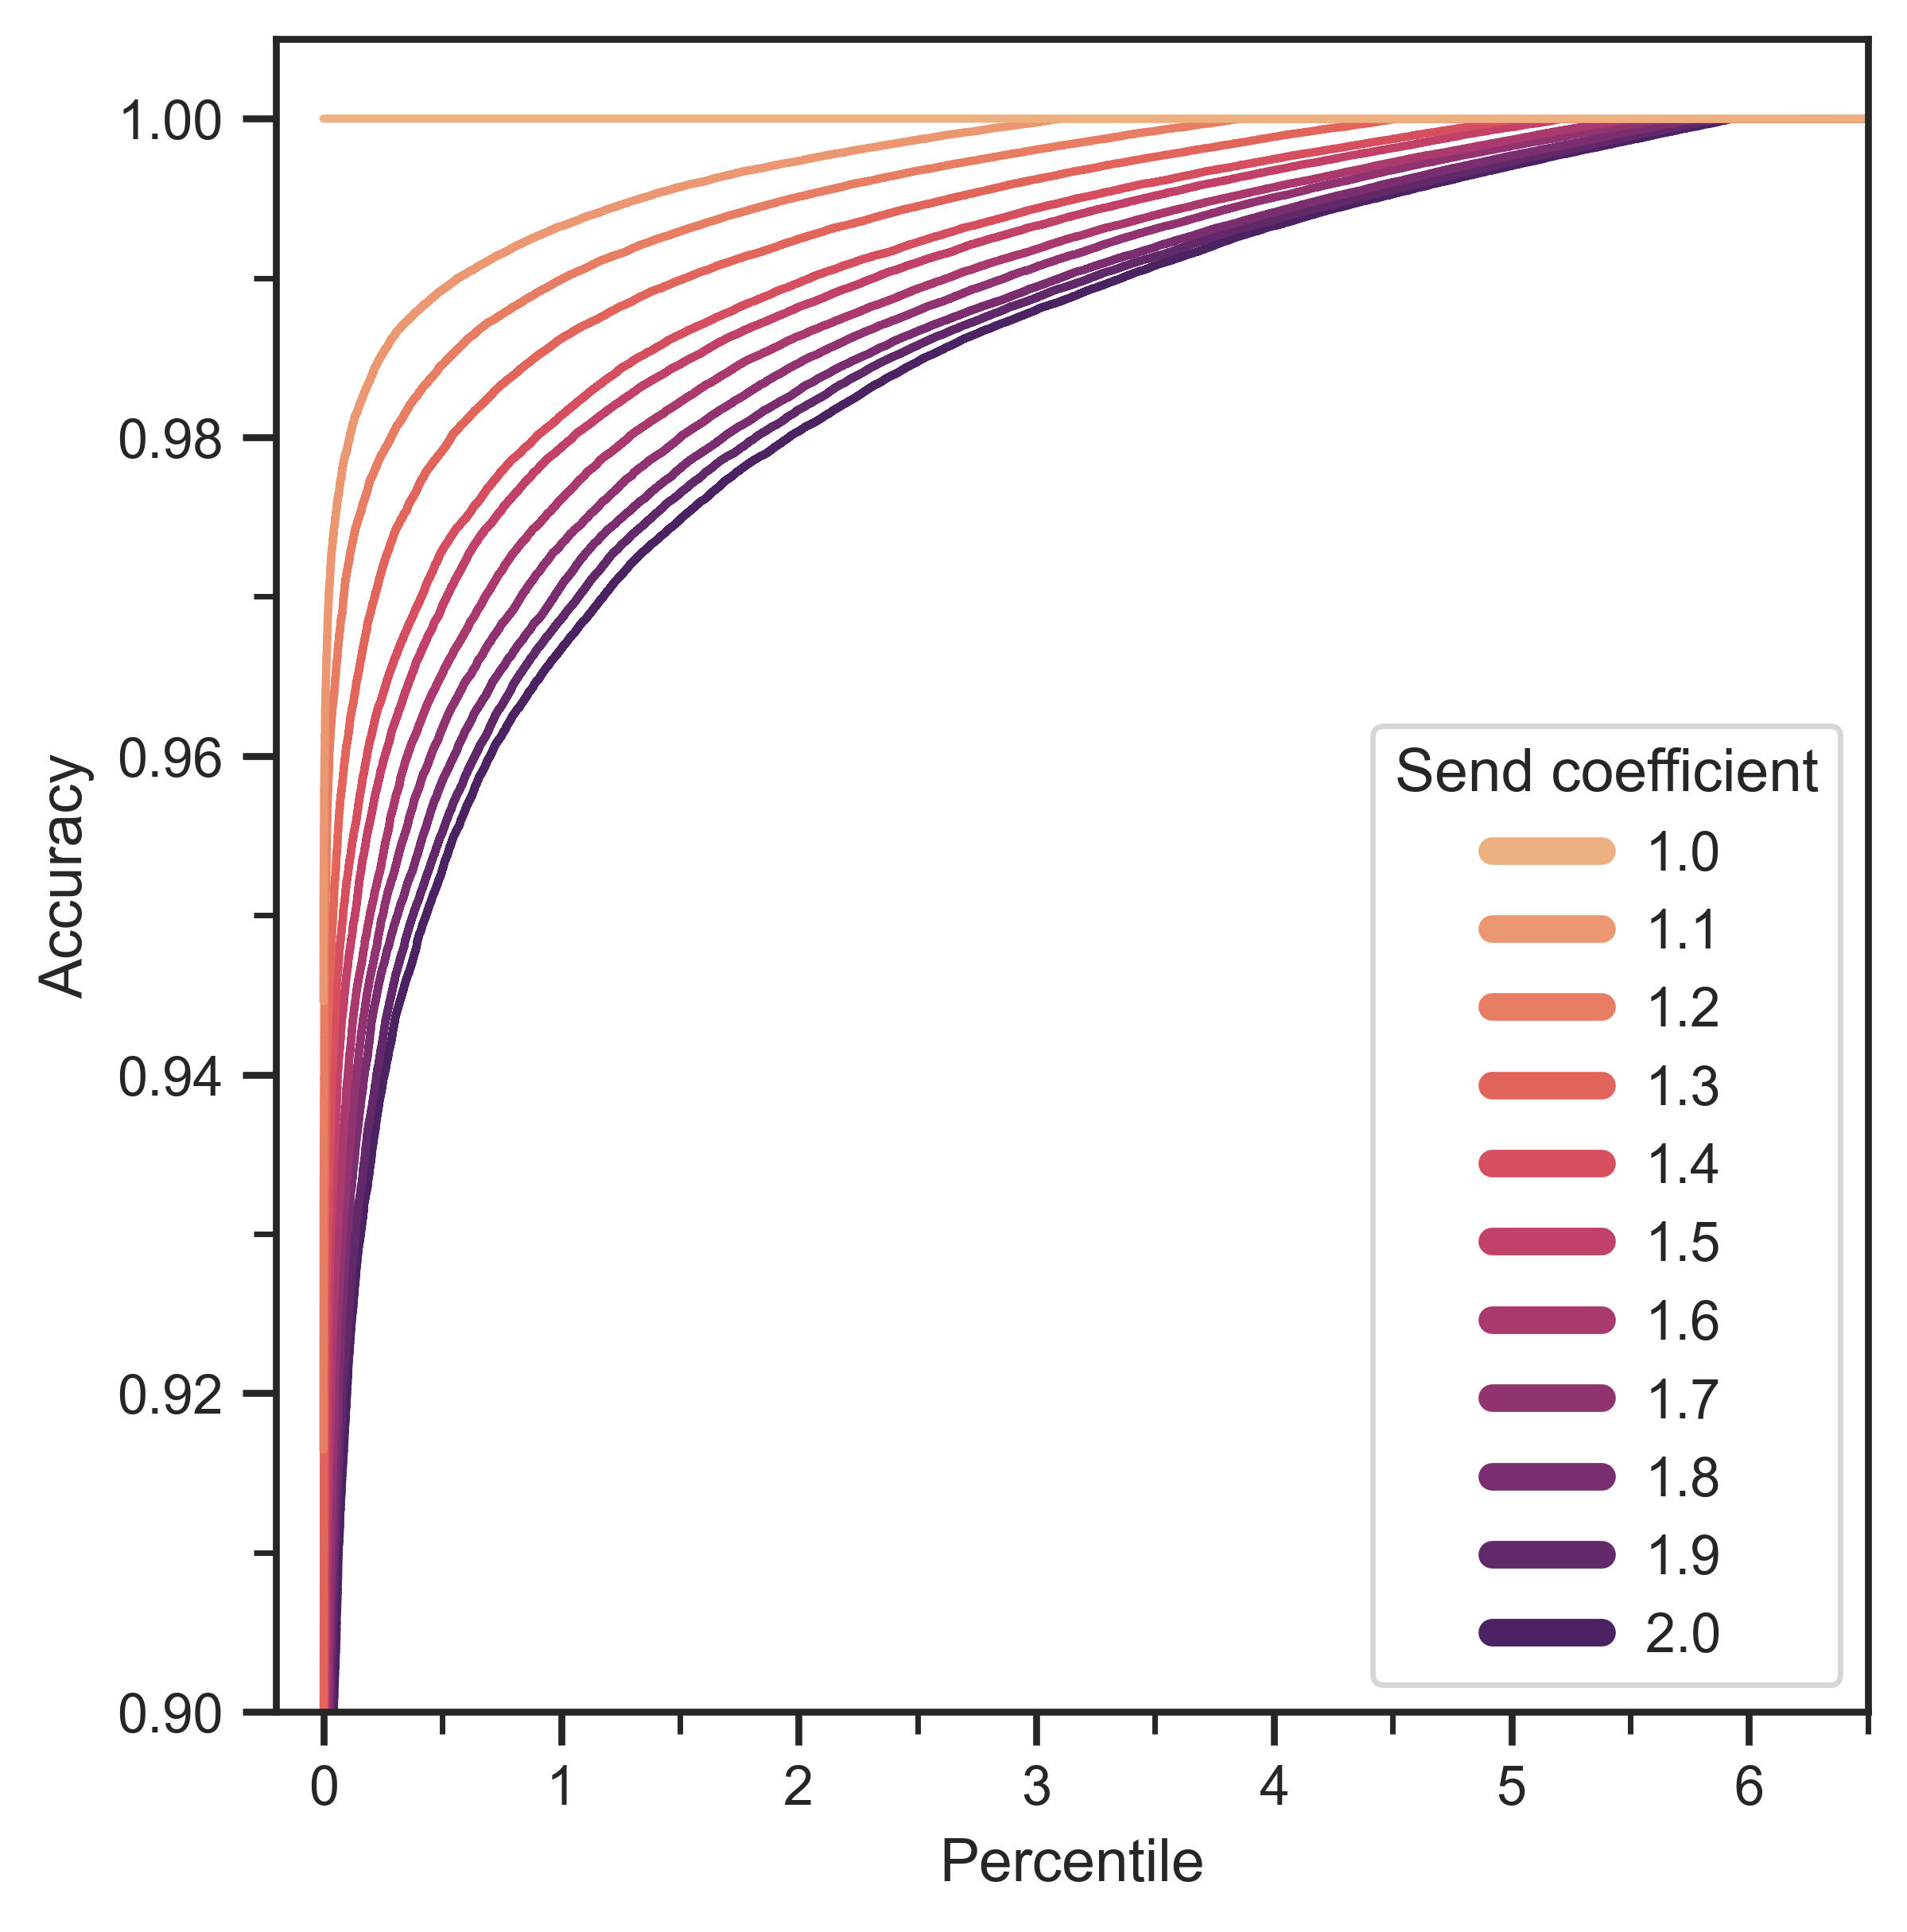
\includegraphics[height=\squareFigHeight]{accuracy-percentiles}
  \caption[Cumulative accuracy distributions]{Cumulative accuracy distributions.}
\end{figure}

\begin{figure}
  \centering
  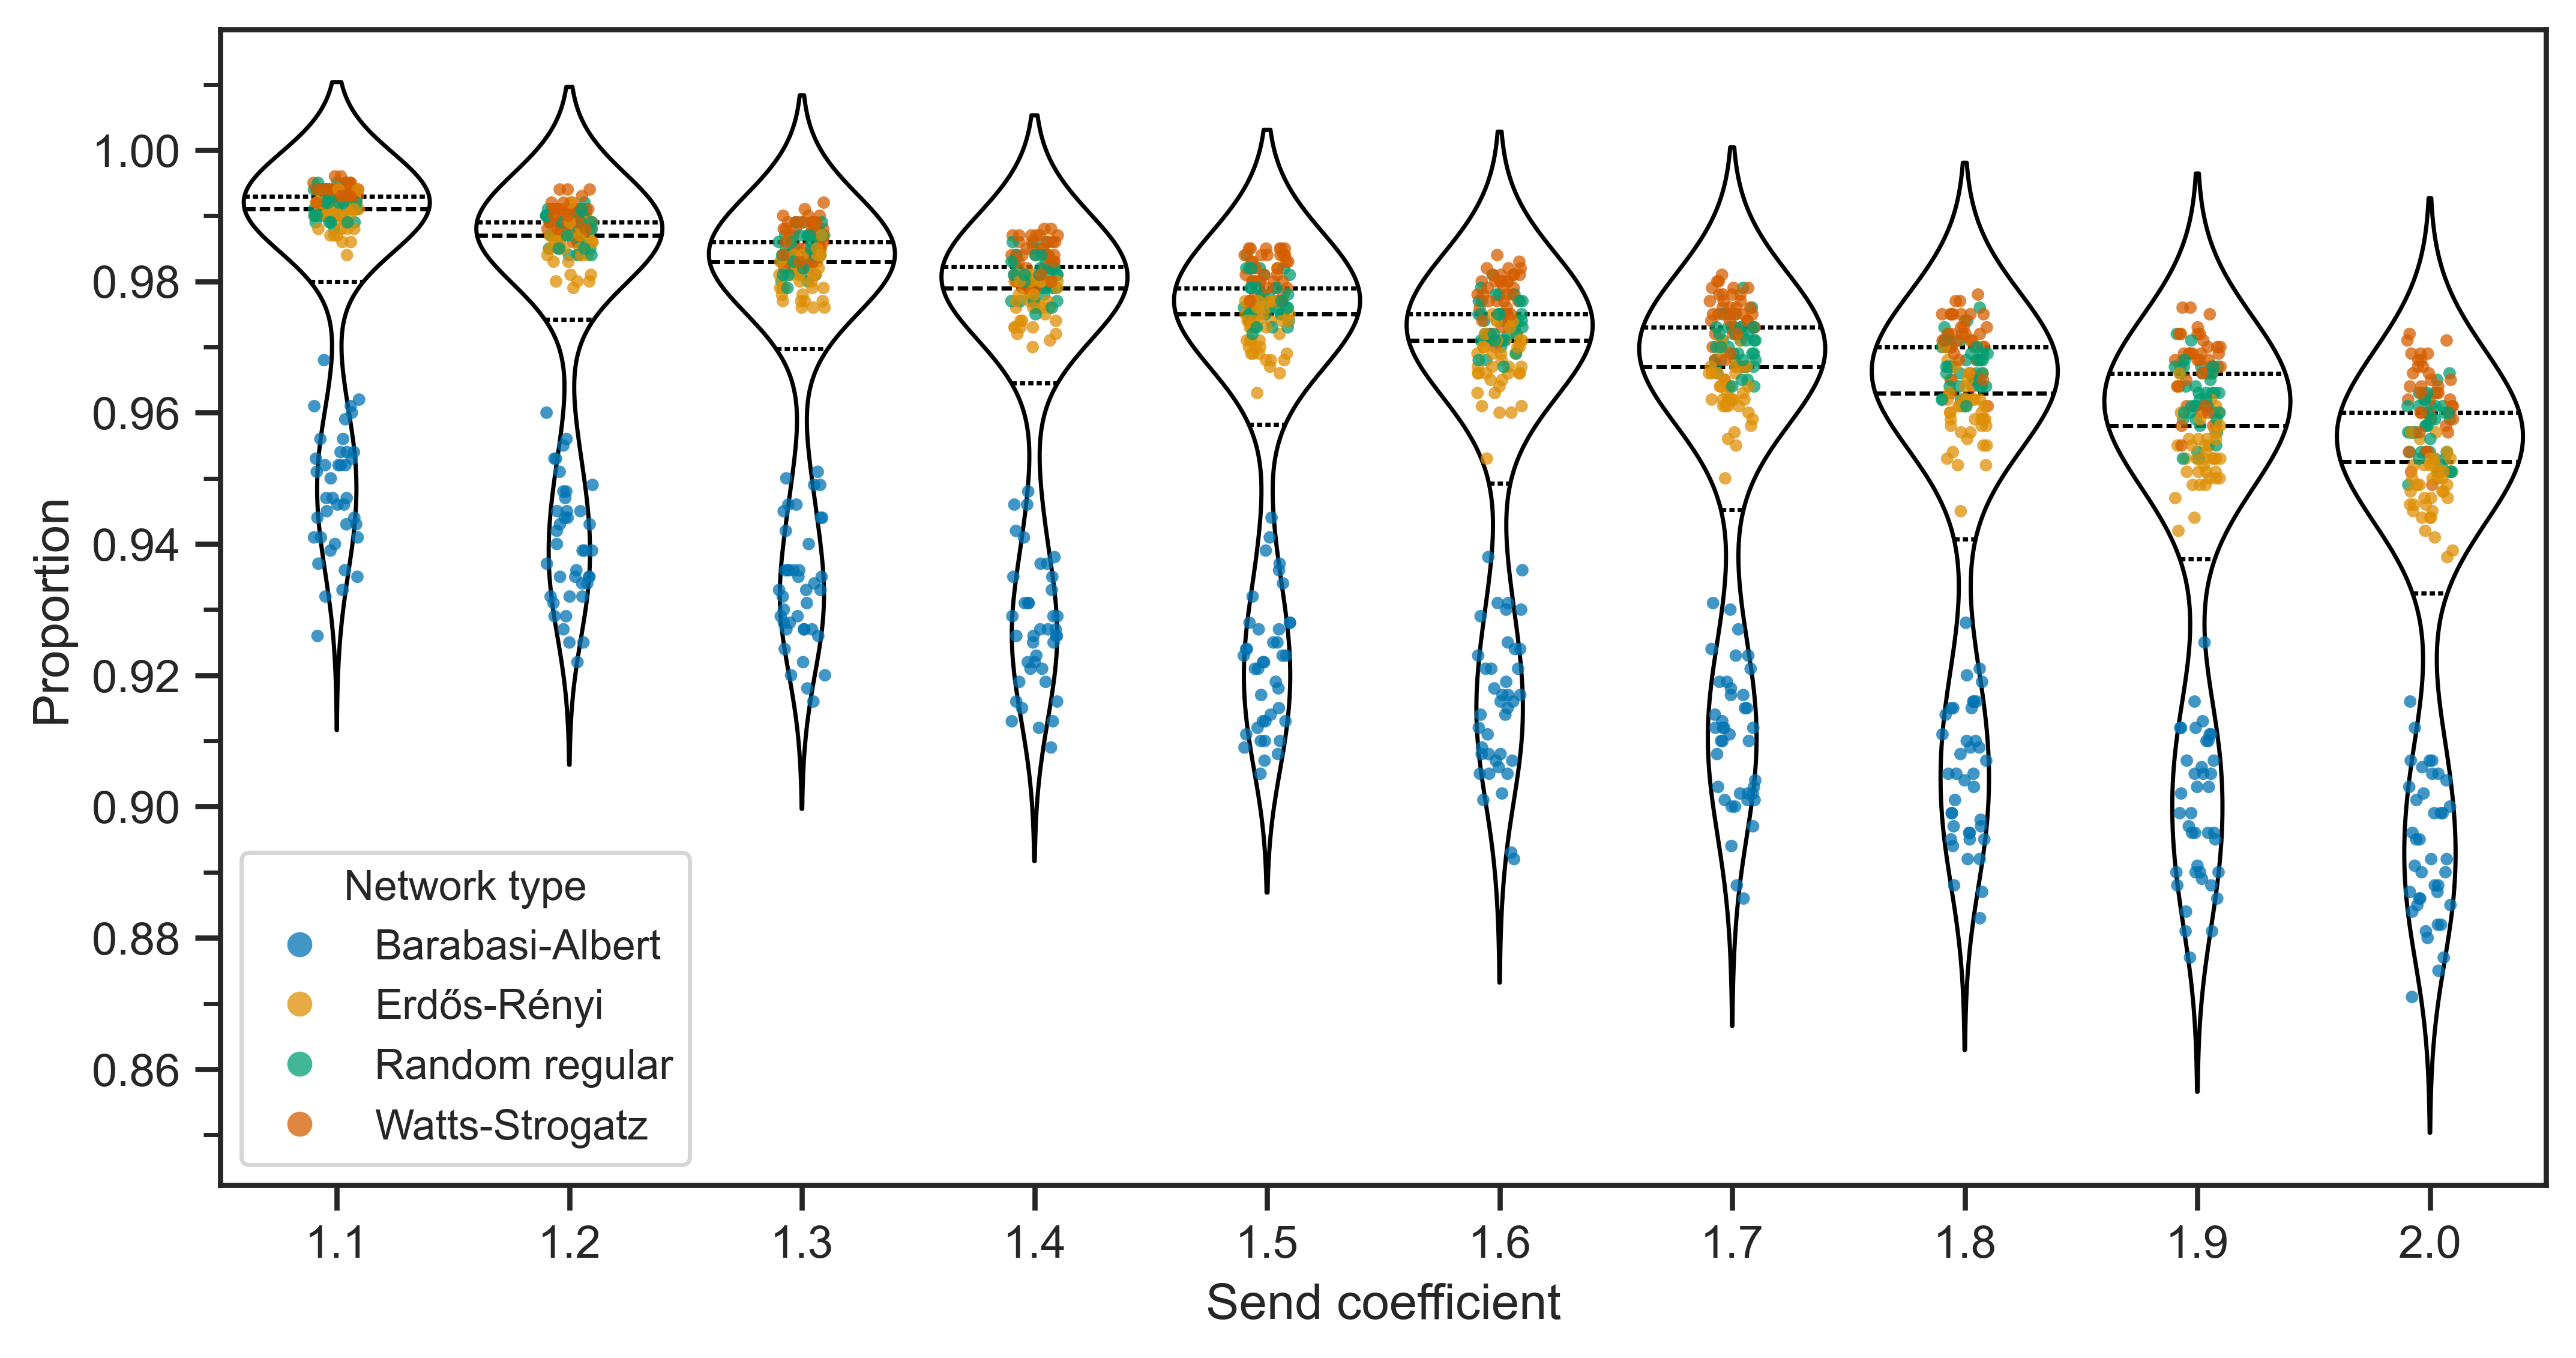
\includegraphics[width=\wideFigWidth]{accuracy-proportions}
  \caption[Send coefficient optimality distributions]{Send coefficient optimality distributions. The dashed line inside each violin marks the median. The upper and lower dotted lines inside each violin mark the upper and lower quartiles, respectively.}
\end{figure}
\end{frame}

\begin{frame}{Experiment 1: Efficiency}
\begin{figure}
  \centering
  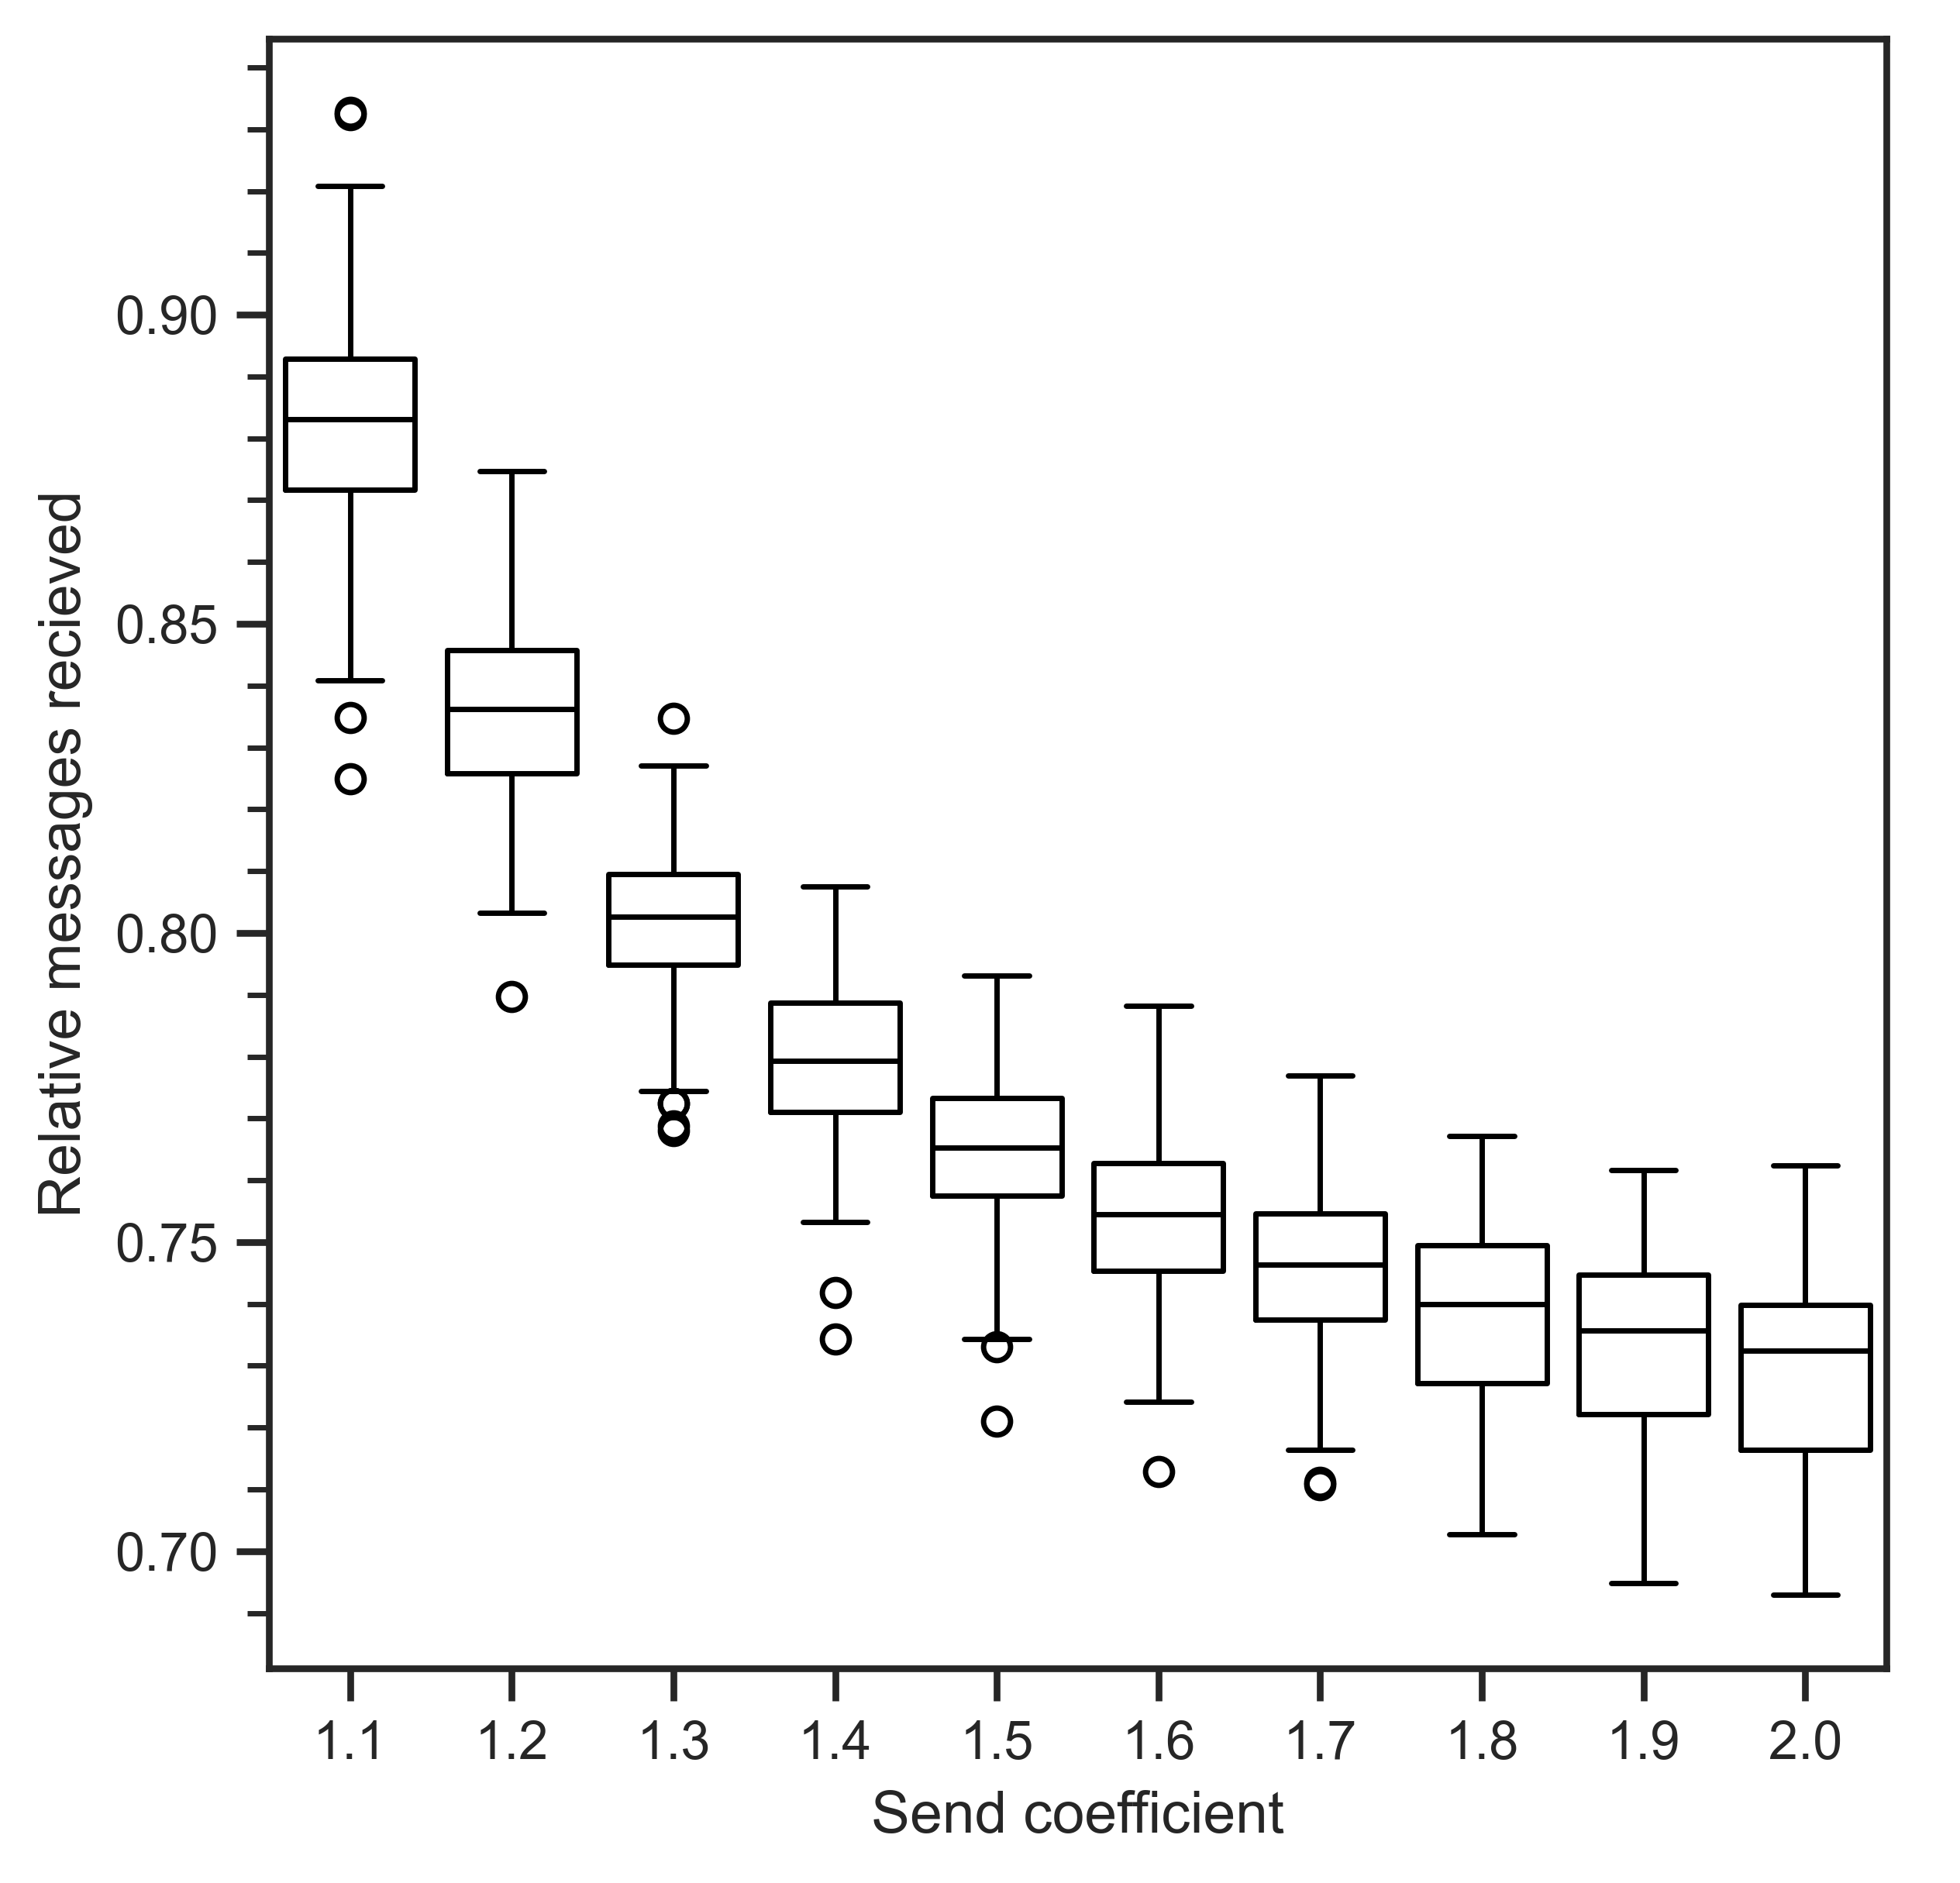
\includegraphics[height=\squareFigHeight]{relative-receives}
  \caption[Message-passing efficiency]{Message-passing efficiency. The send coefficient $\pSendCoefficient = 1$ was used as a baseline for message-passing efficiency since it was found to be the maximum send coefficient that achieves perfect accuracy.}
\end{figure}

%\begin{figure}
%  \centering
%  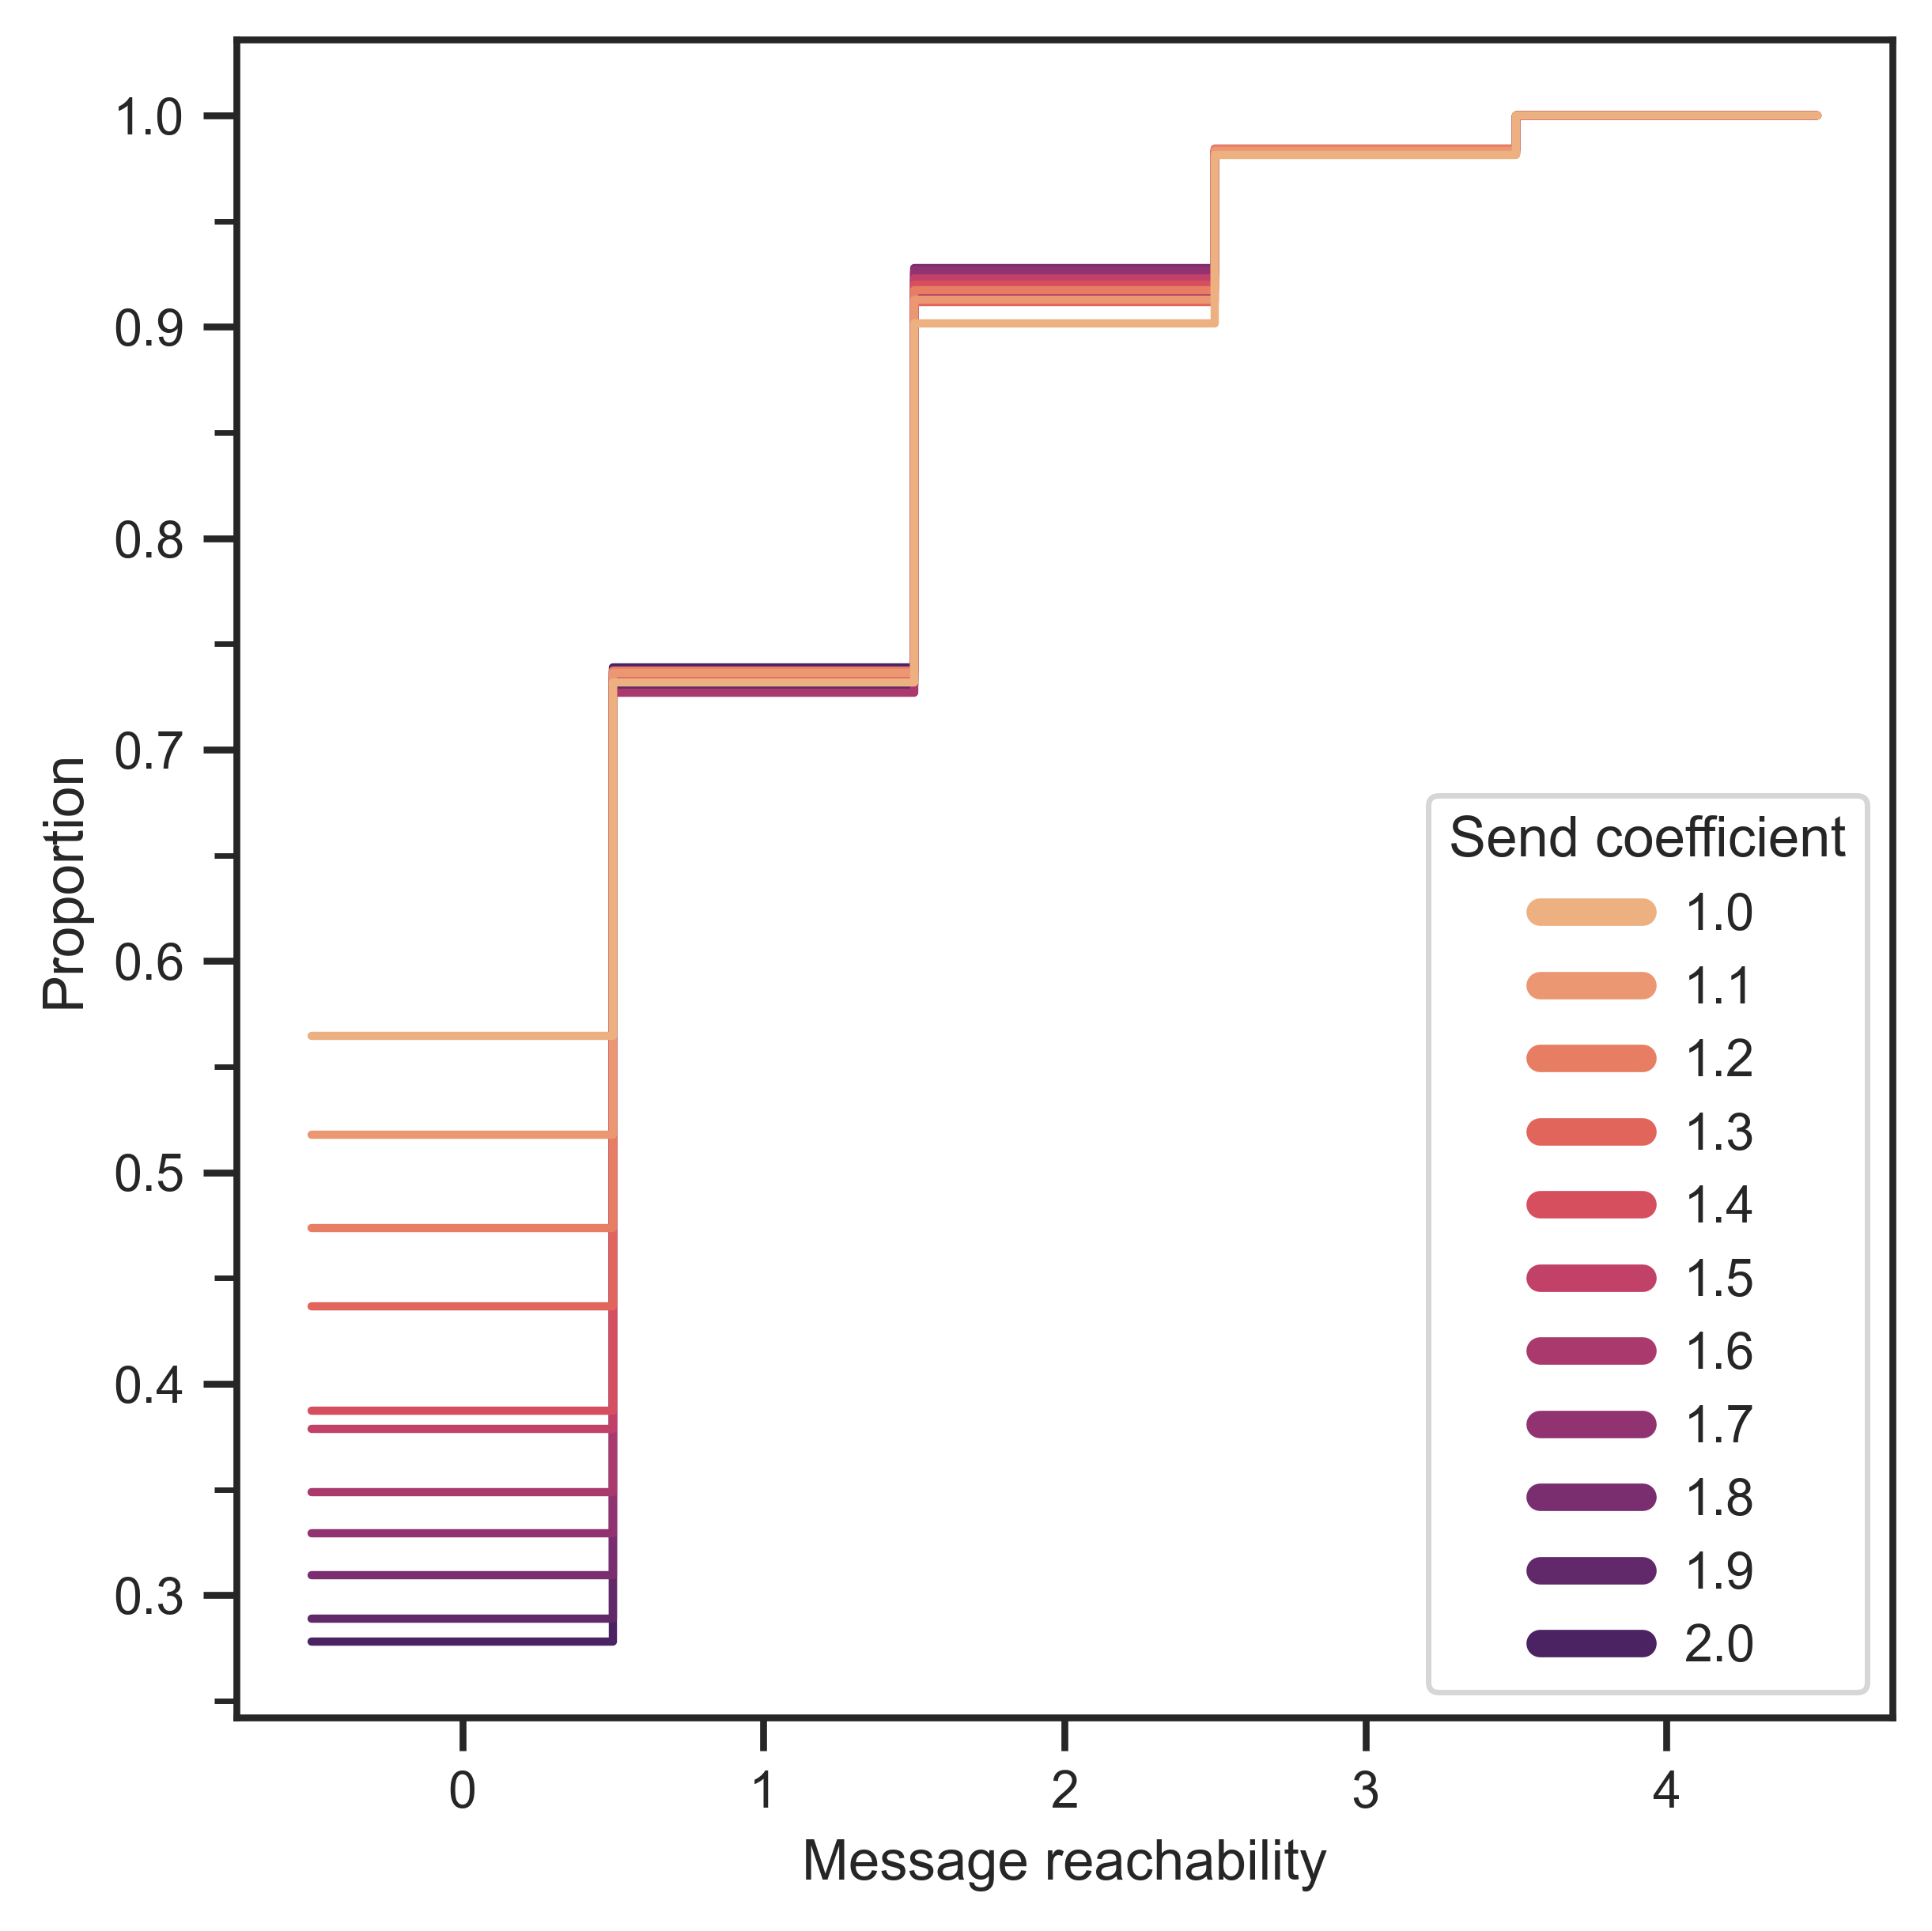
\includegraphics[height=\squareFigHeight]{message-reachability}
%  \caption[Message reachability cumulative distributions]{Message reachability cumulative distributions.}
%\end{figure}
\end{frame}

\begin{frame}[allowframebreaks]{Experiment 1: Exploration}
\begin{figure}
  \centering
  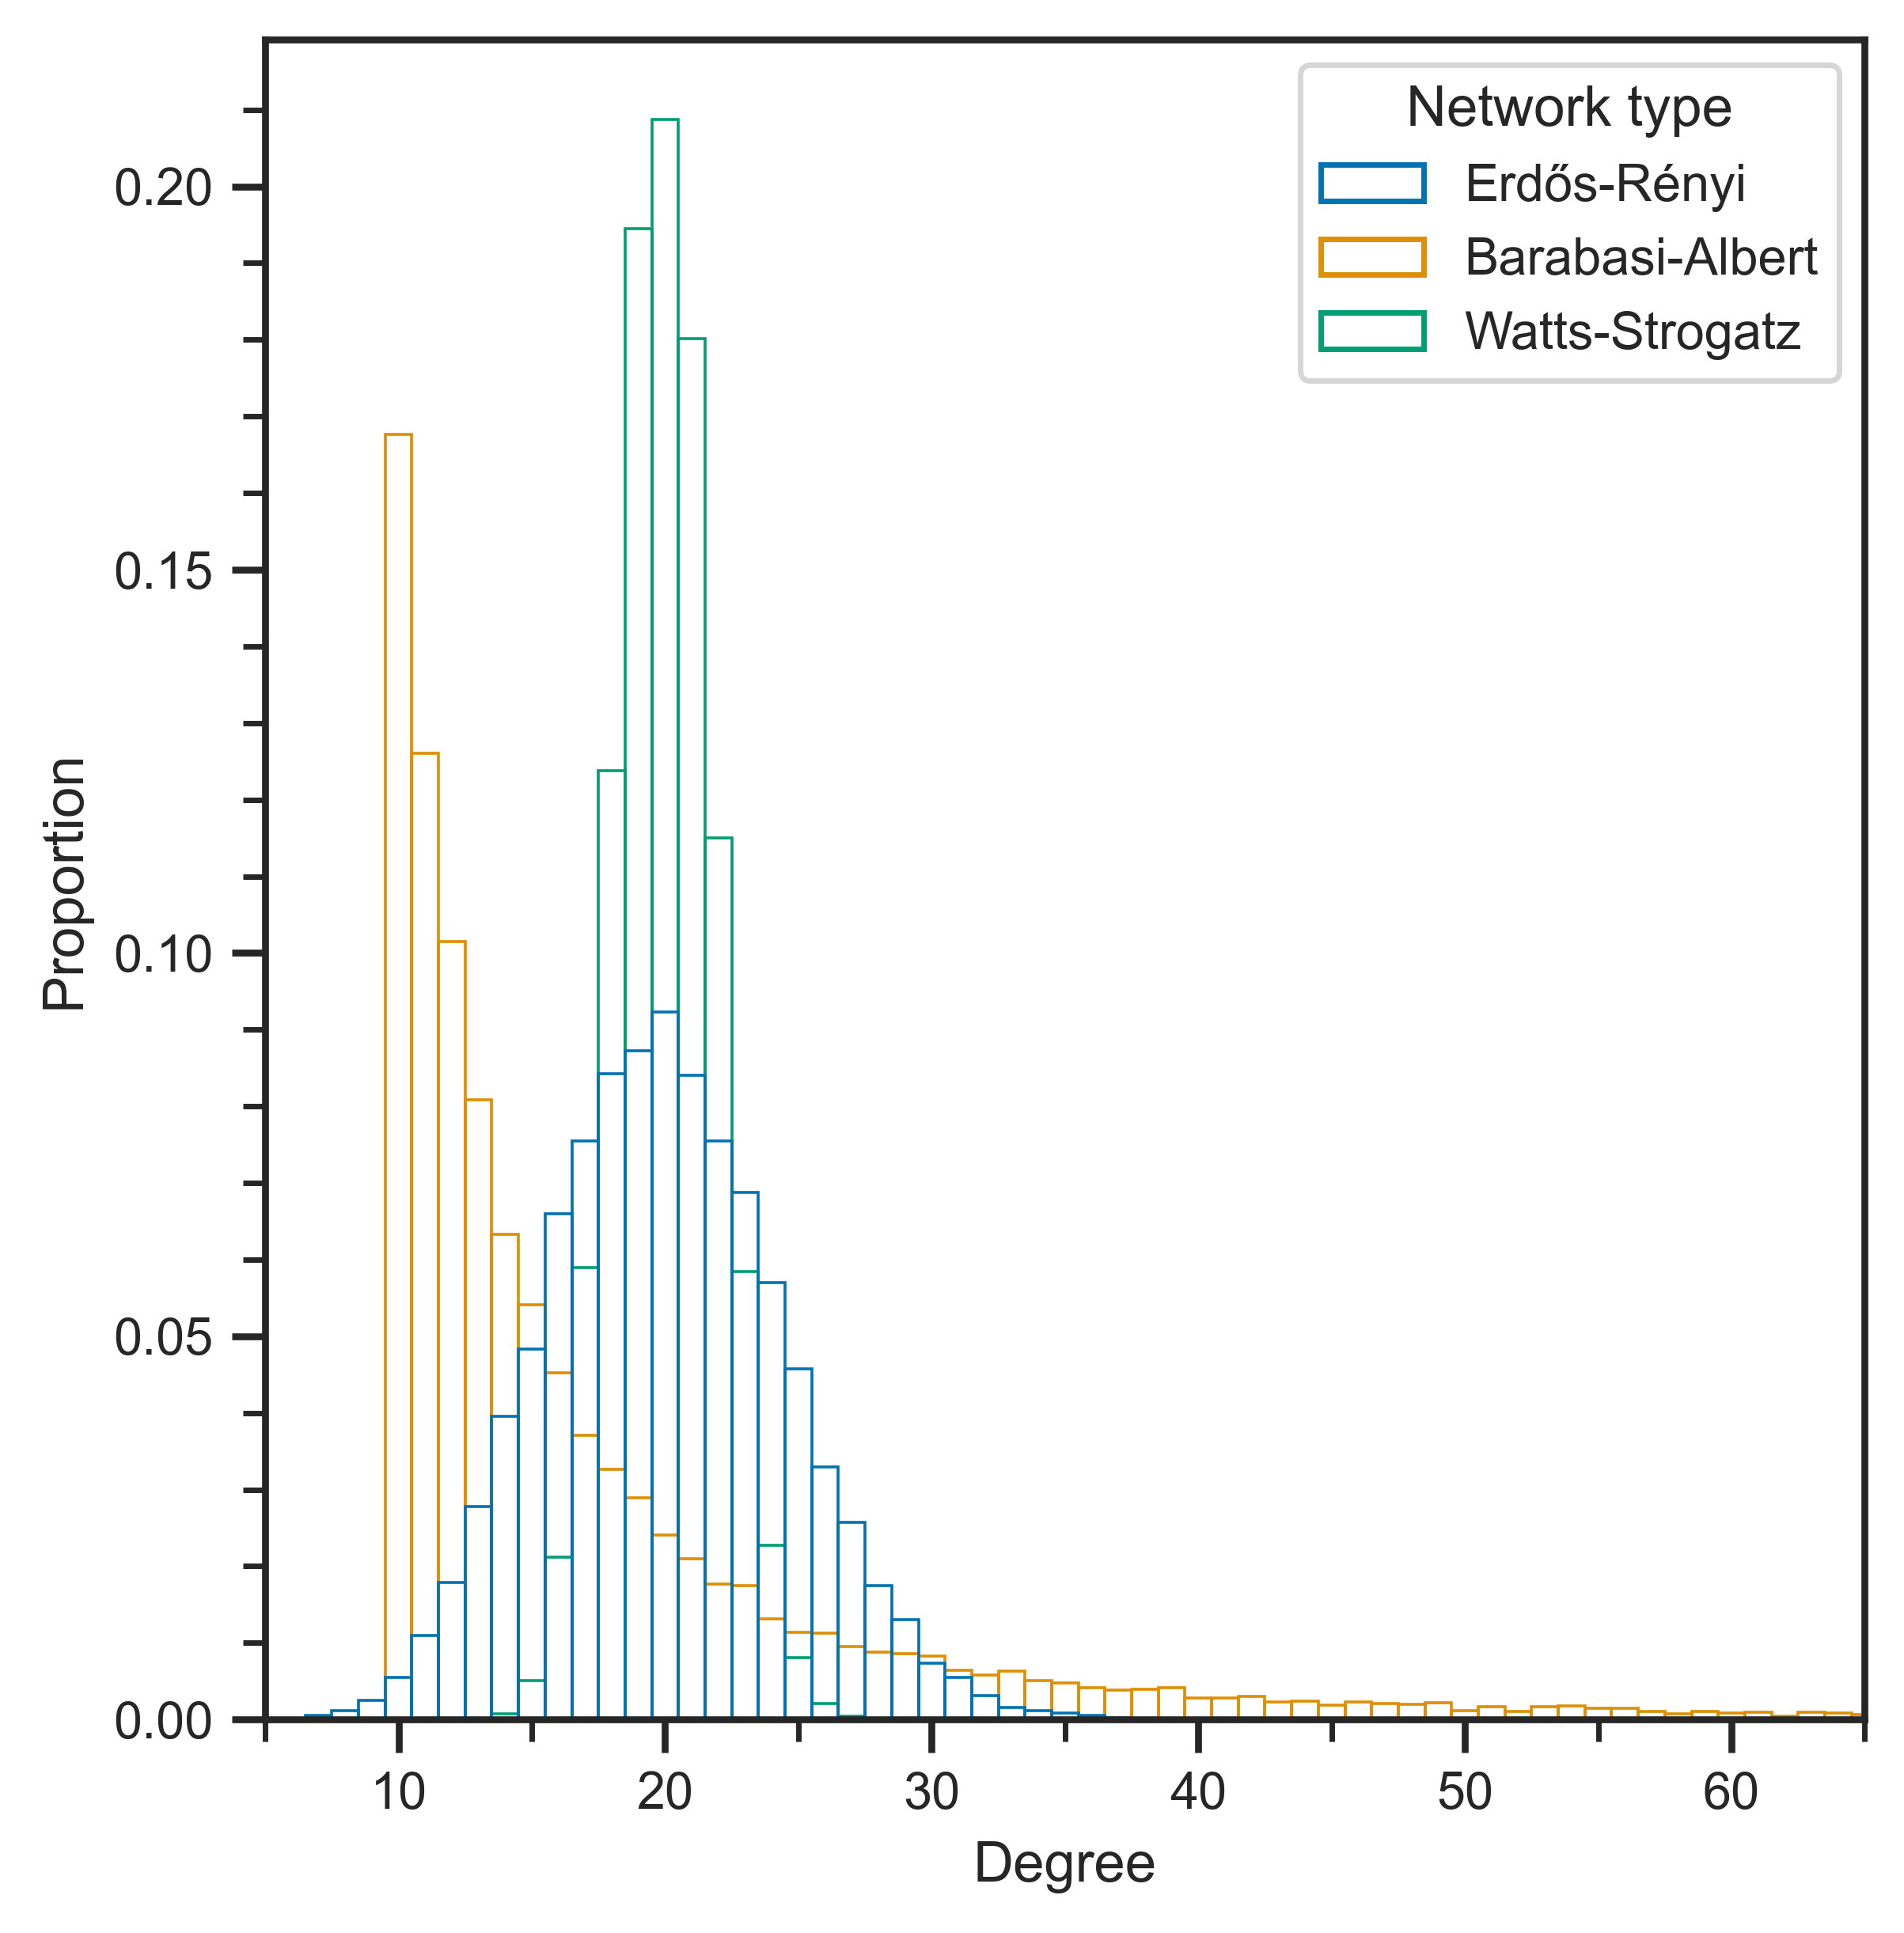
\includegraphics[height=\squareFigHeight]{network-degree-distributions}
  \caption[Contact network degree distributions]{Contact network degree distributions. All vertices in random regular contact networks had a degree of 20, so the distribution was omitted to provide more visual space for the distributions of other contact networks.}
\end{figure}

\begin{figure}
  \centering
  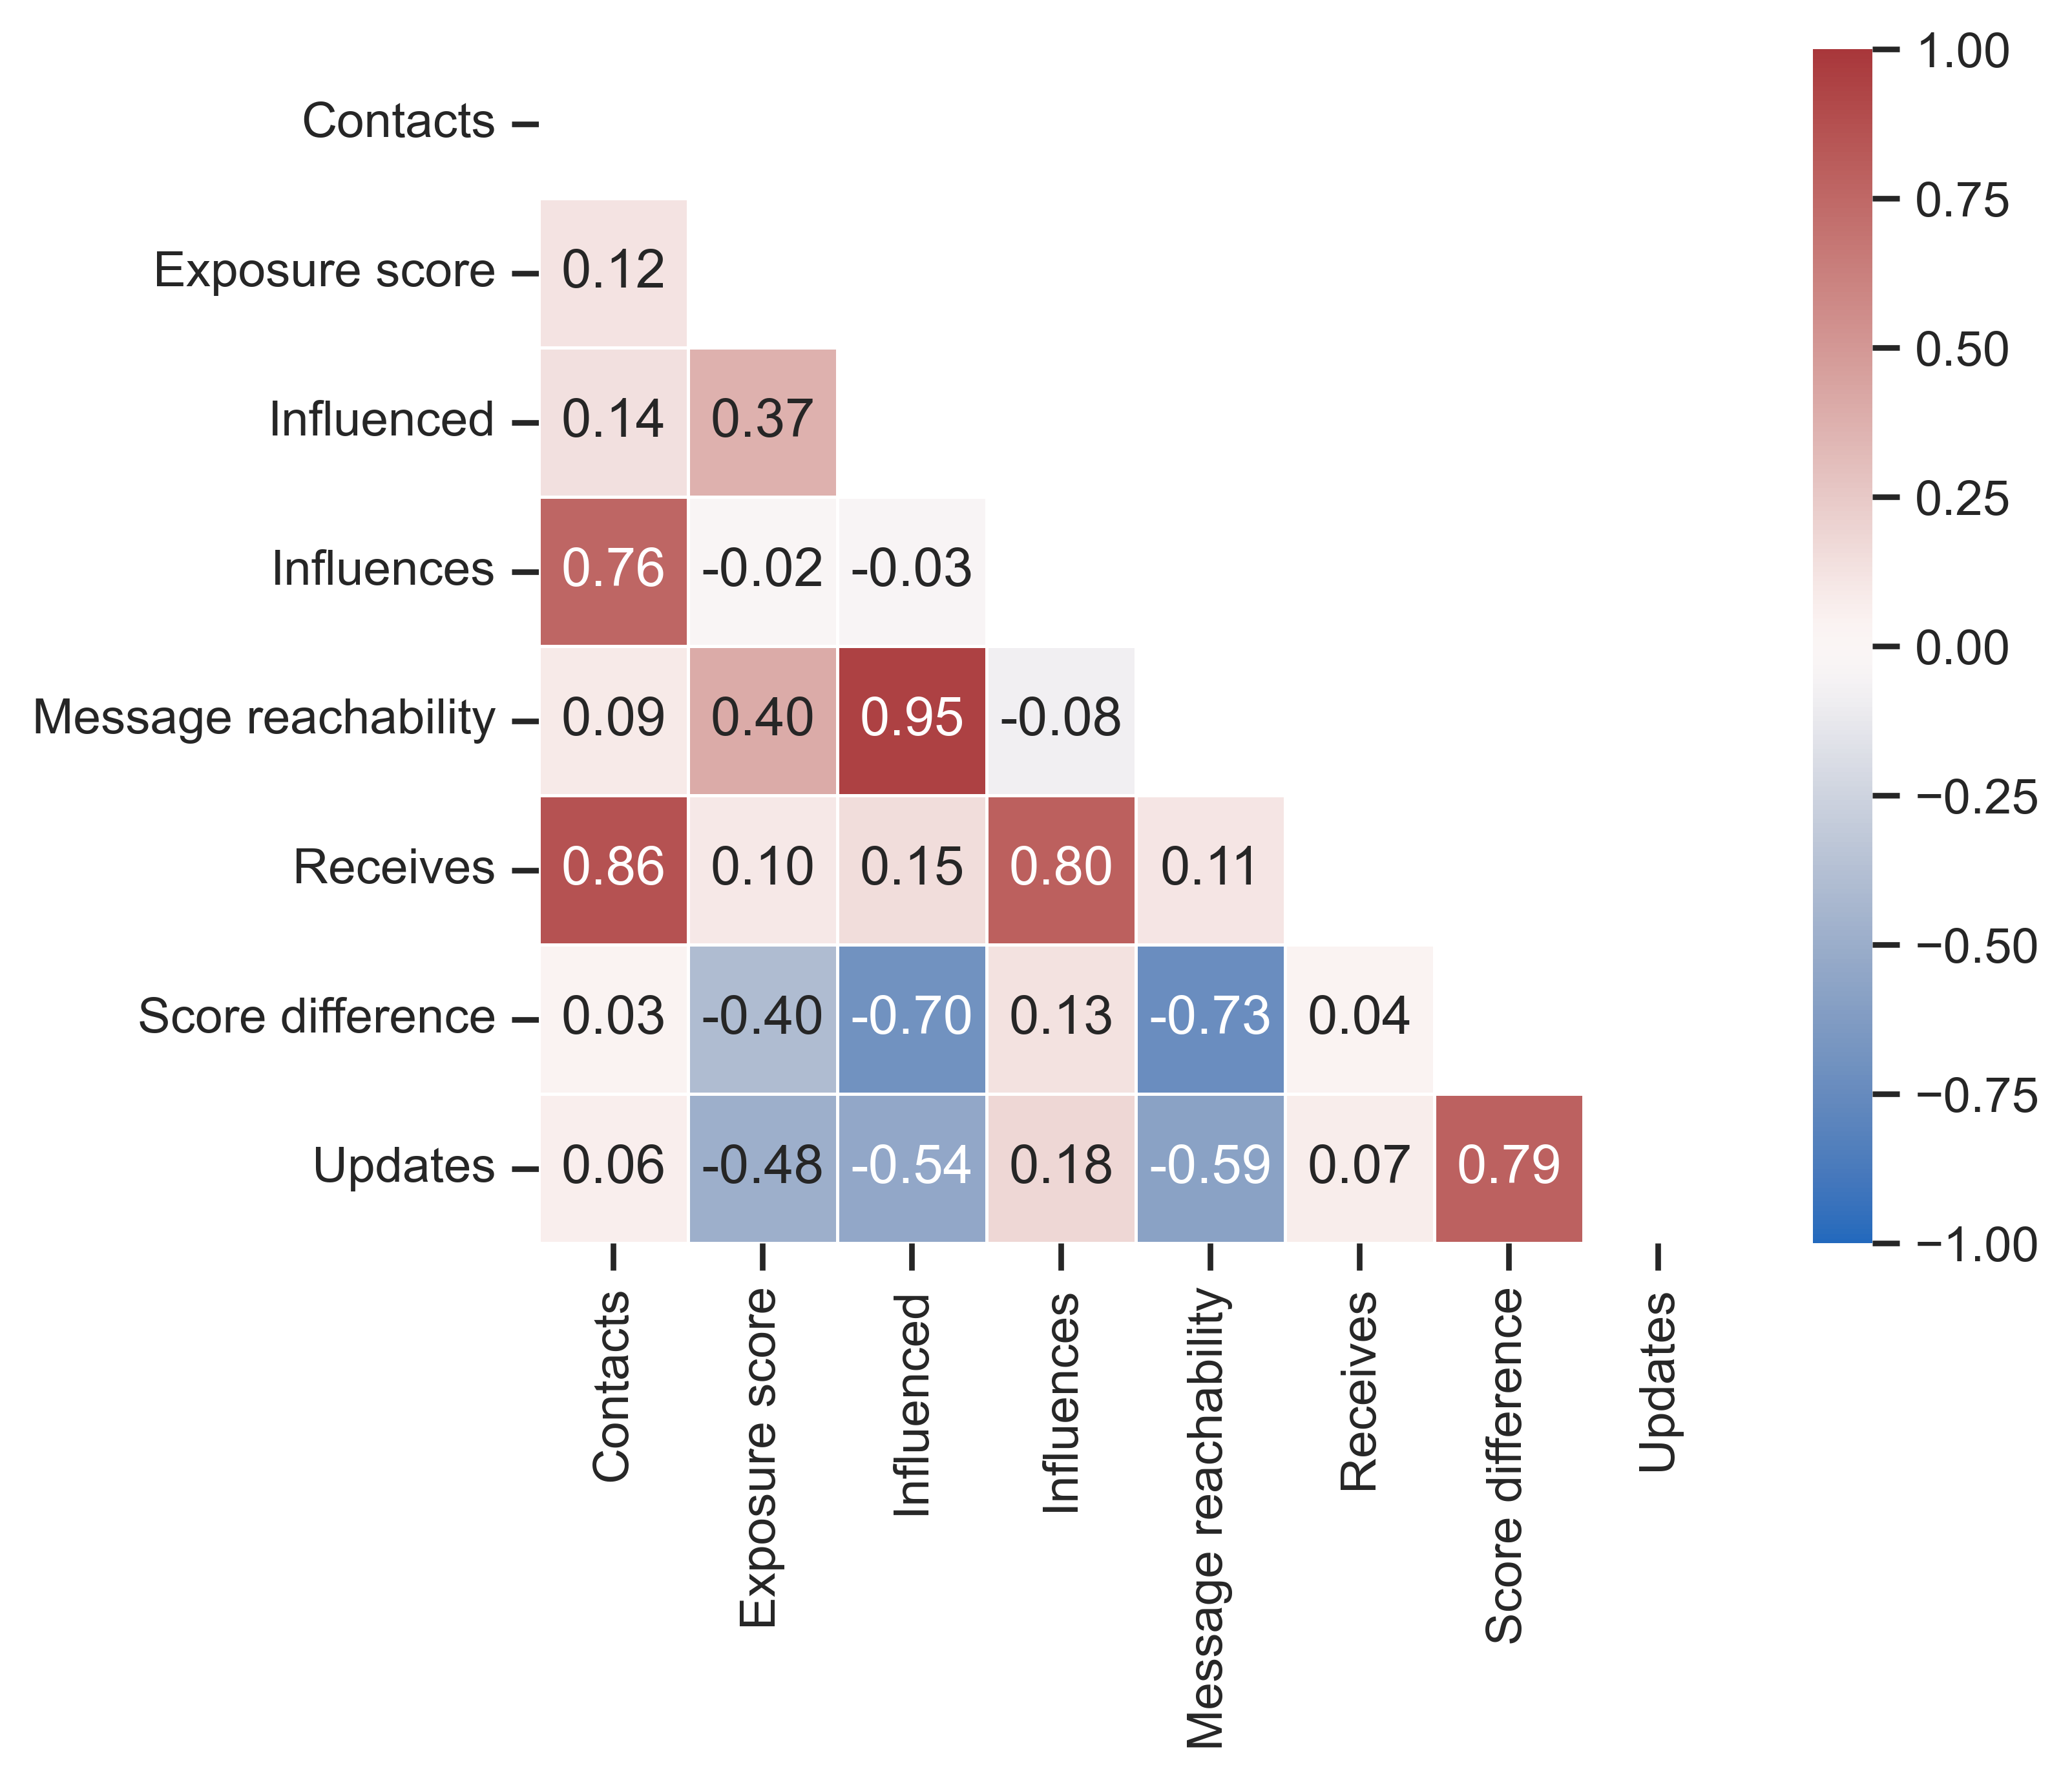
\includegraphics[height=\squareFigHeight]{correlation}
  \caption[Correlation matrix of dataset attributes]{Correlation matrix of dataset attributes. Each cell is the Spearman rank partial correlation coefficient \citep{Spearman1904}, controlling for the effect of the send coefficient. All coefficients are significant ($p < 0.01$), adjusting for multiple comparisons via the Holm–Bonferroni method \citep{Holm1979}.}
\end{figure}
\end{frame}

\begin{frame}{Experiment 2: Benchmarking Hypothesis Testing}
\end{frame}

\begin{frame}[allowframebreaks]{Experiment 3: Benchmarking}
\begin{figure}
  \centering
  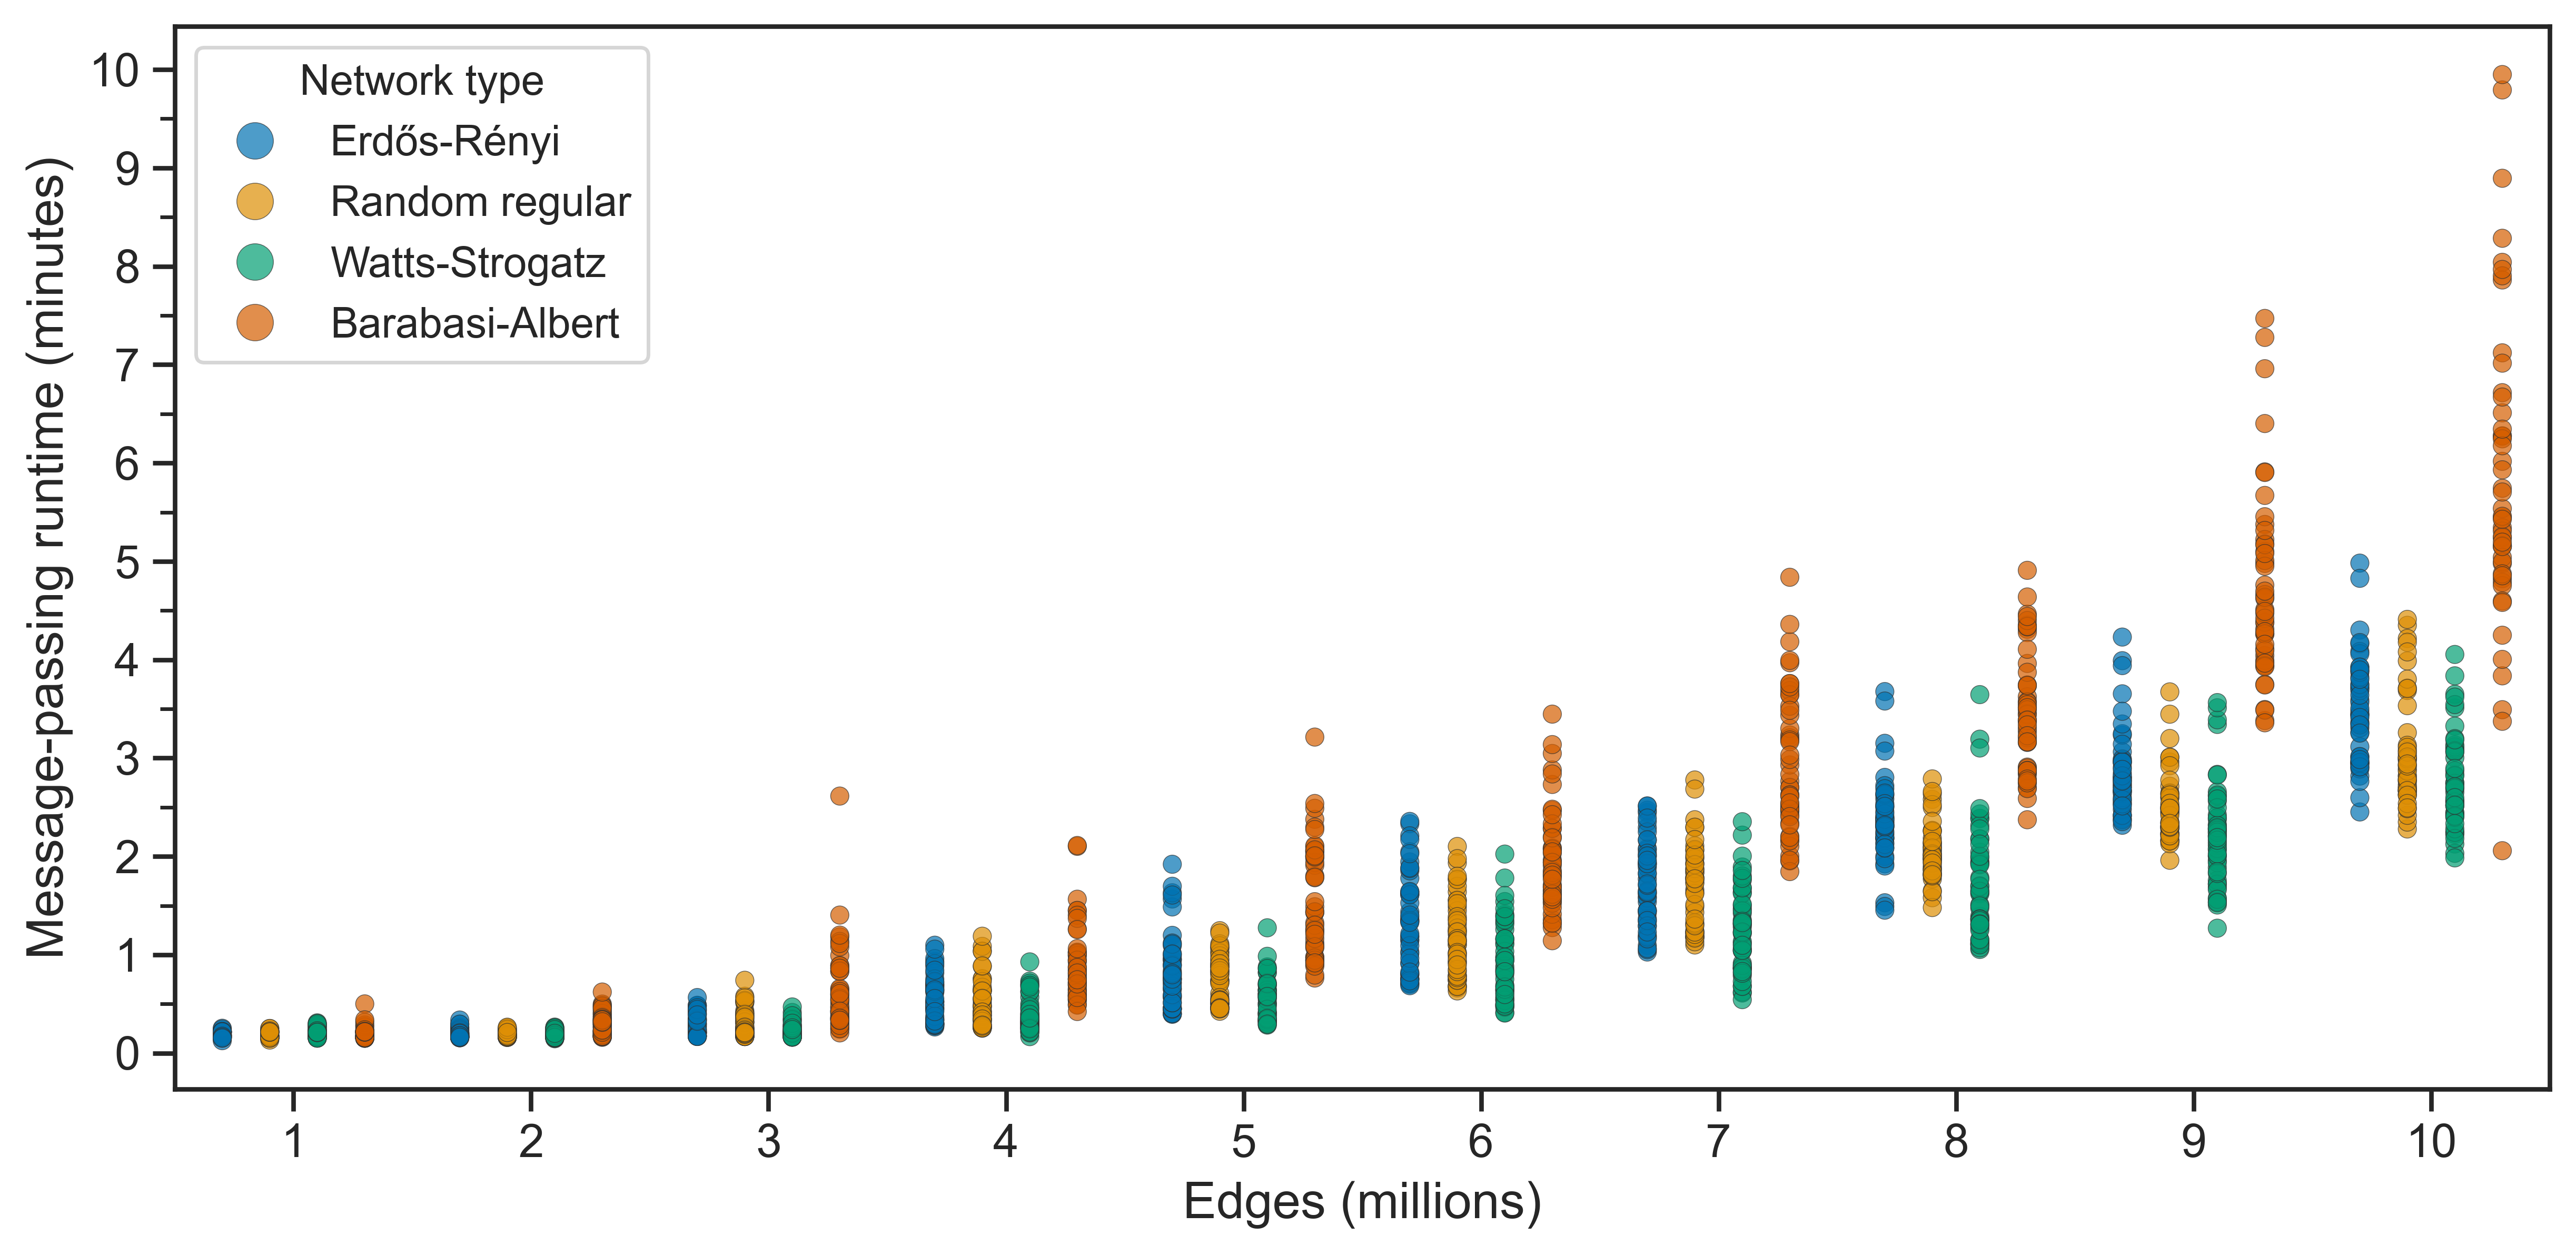
\includegraphics[width=\wideFigWidth]{runtimes}
  \caption[Message-passing runtimes]{Message-passing runtimes.}
\end{figure}

\begin{figure}
  \centering
  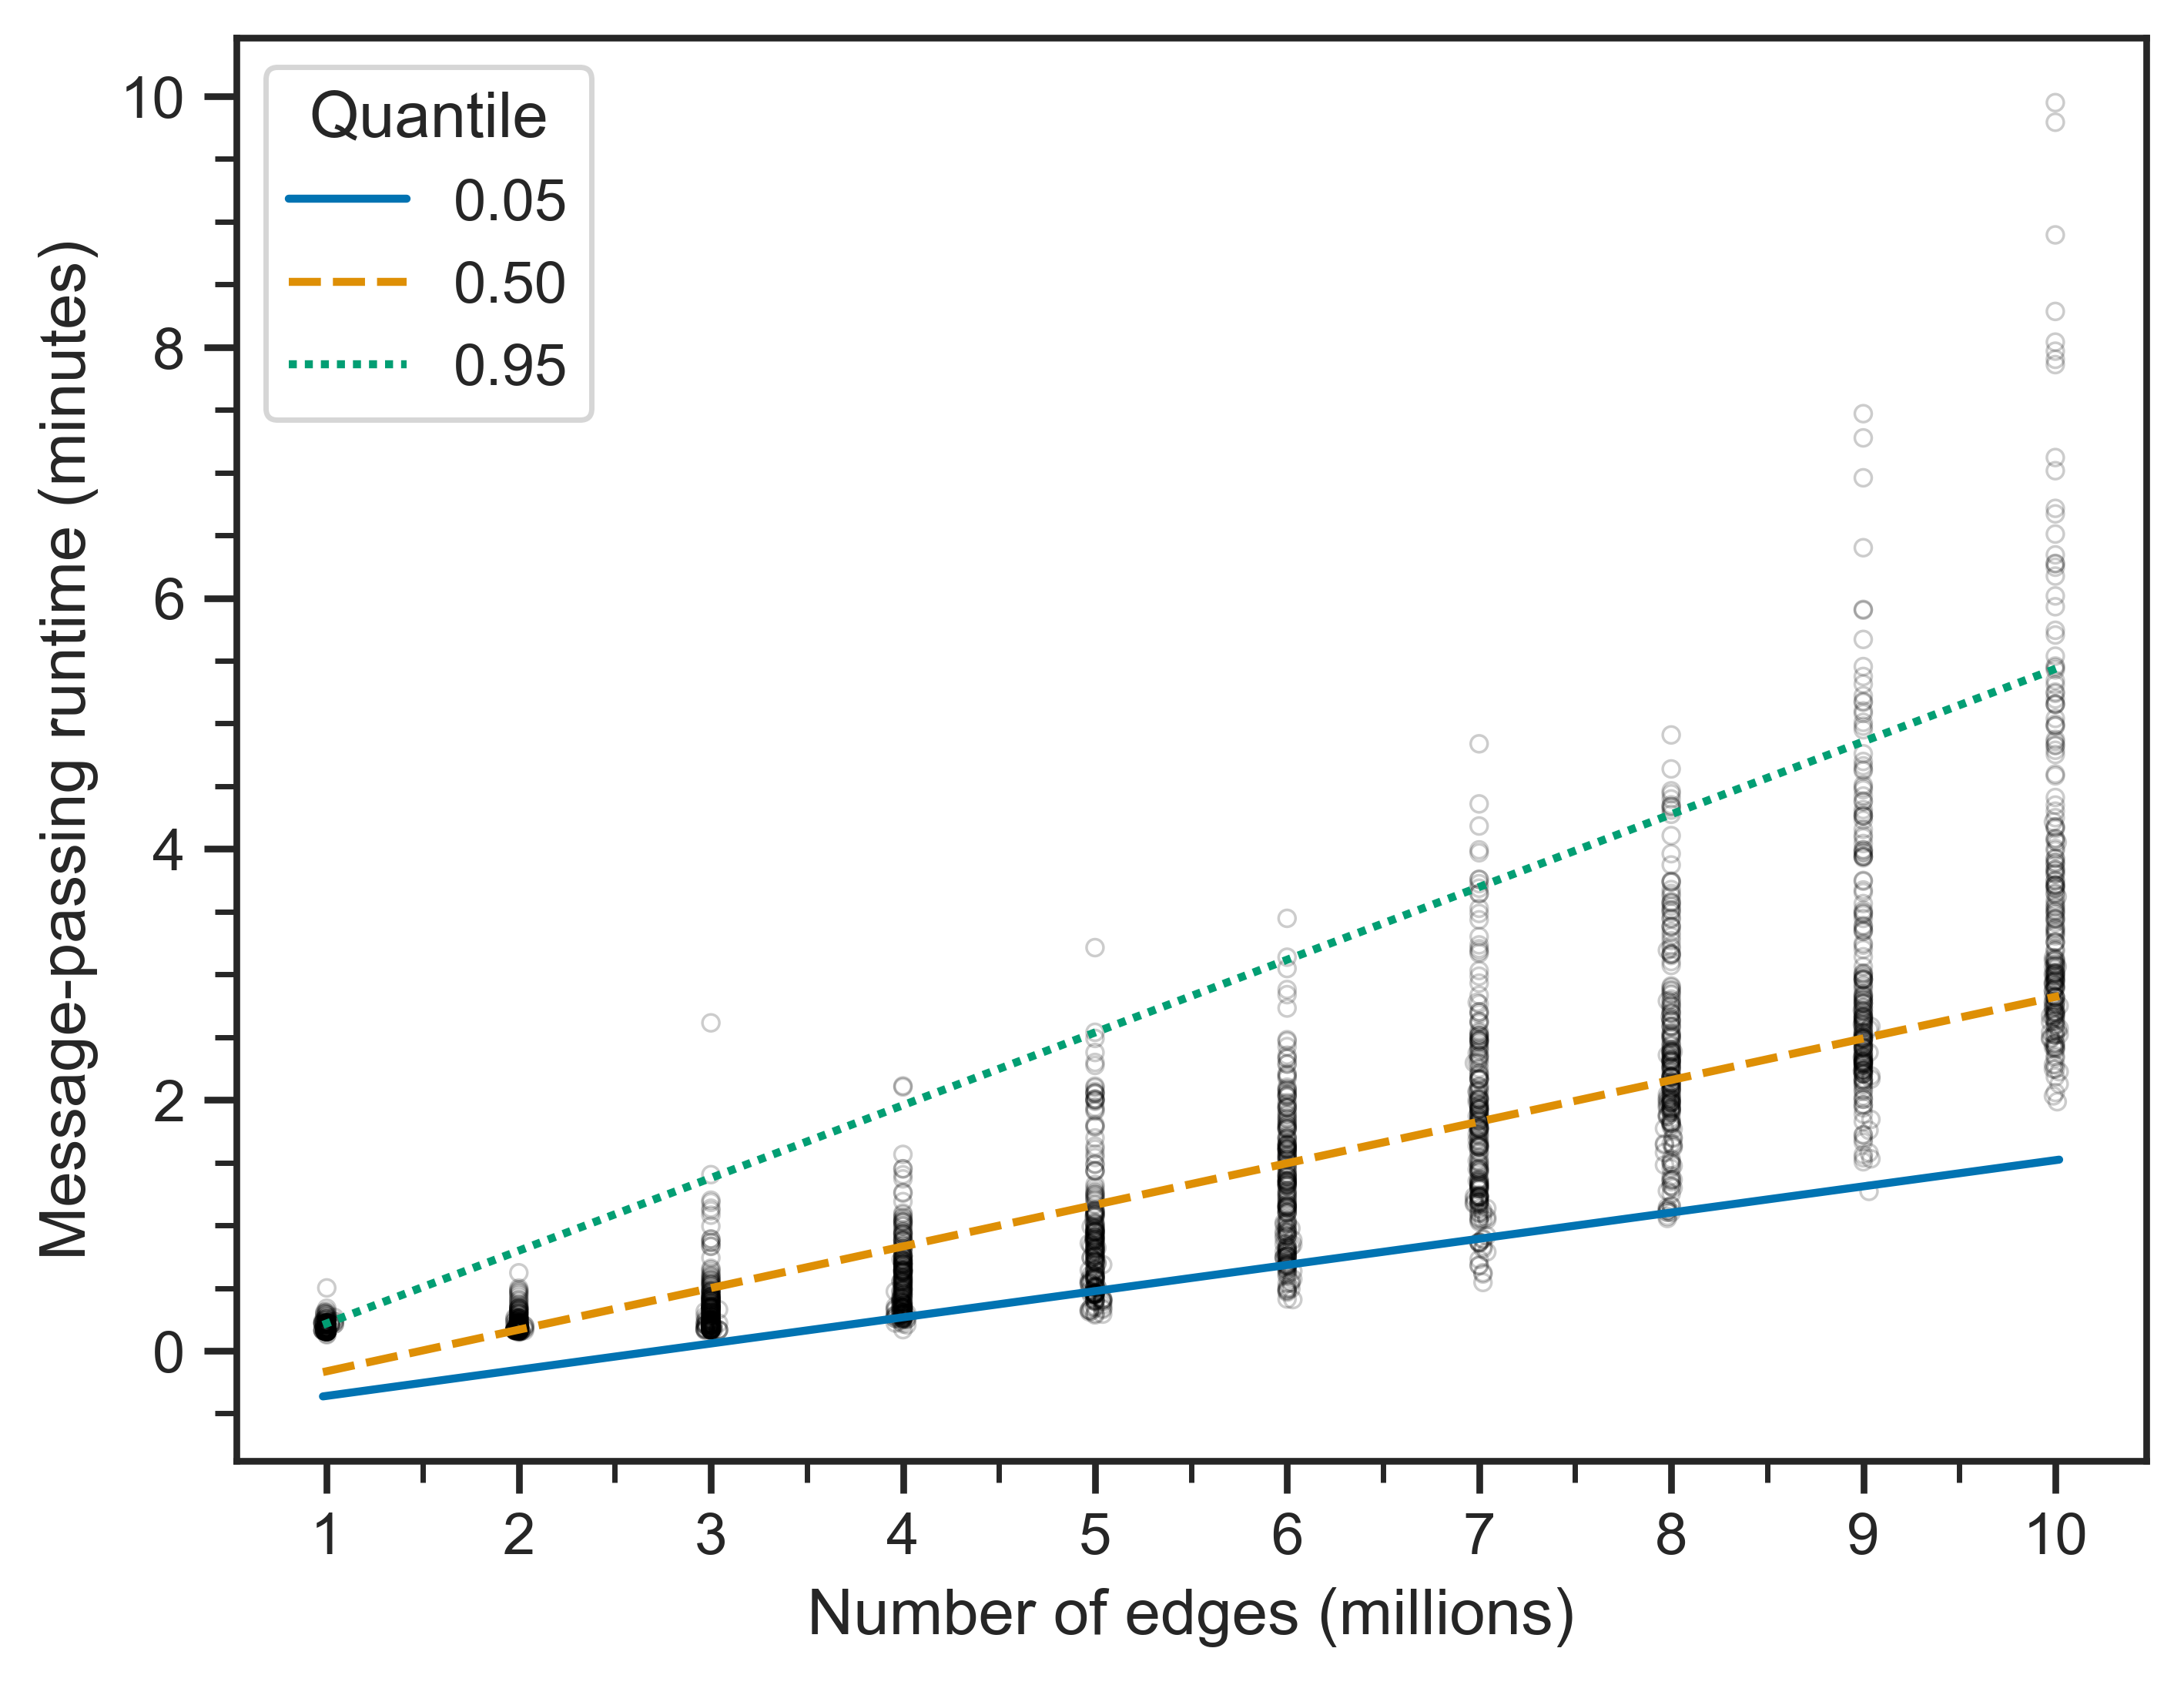
\includegraphics[height=\squareFigHeight]{runtime-regression}
  \caption[Message-passing runtimes with regression lines]{Message-passing runtimes with regression lines.}
\end{figure}
\end{frame}

\end{section}

\begin{section}{Conclusion}

\begin{frame}{Conclusion: Future Work}
\begin{itemize}
  \item Incorporate differential privacy techniques that are designed for DCT applications that utilize risk scores \citep{Romijnders2024}.
  \pause
  \item Formally define the security and privacy characteristics of ShareTrace, using the framework proposed by \citet{Kuhn2021} to characterize the latter.
  \pause
  \item Conduct a simulation-based analysis of asynchronous risk propagation with COVI-AgentSim \citep{Gupta2020}.
  \pause
  \item Explore the utility and feasibility of integrating decentralized technologies \citep{Benet2014, Troncoso2017, Trautwein2022, Shi2024, Keizer2024} and self-soverign identity \citep{Preukschat2021, Schardong2022} into the system design.
\end{itemize}
\end{frame}


\end{section}

% A section is automatically created for references.
\begin{frame}[allowframebreaks]{References}
  \printbibliography
\end{frame}

\end{document}